\documentclass{article}

\usepackage{amsmath,amssymb}
\usepackage{tikz}
\usepackage{pgfplots}
\usepackage{xcolor}
\usepackage[left=2.1cm,right=3.1cm,bottom=3cm,footskip=0.75cm,headsep=0.5cm]{geometry}
\usepackage{enumerate}
\usepackage{enumitem}
\usepackage{marvosym}
\usepackage{tabularx}
\usepackage{hyperref}
\usepackage{varwidth}
\usepackage{parskip}
\usepackage[onehalfspacing]{setspace}

\usepackage{pgfplots}
\pgfplotsset{compat=1.10}
\usepgfplotslibrary{fillbetween}
\usepackage{pgf}
\usepackage{tikz}
\usepackage{tikz-qtree}
\usetikzlibrary{patterns,arrows,calc,decorations.pathmorphing,backgrounds, positioning,fit,petri,decorations.fractals,trees,cd,automata,babel,shapes.geometric,arrows.meta,bending}


\usepackage{listings}
\definecolor{lightlightgray}{rgb}{0.95,0.95,0.95}
\definecolor{lila}{rgb}{0.8,0,0.8}
\definecolor{mygray}{rgb}{0.5,0.5,0.5}
\definecolor{mygreen}{rgb}{0,0.8,0.26}
\lstdefinestyle{R} {language=R,morekeywords={confint,head,fitdist,ks,test}}
\lstset{language=R,
	basicstyle=\ttfamily,
	keywordstyle=\color{lila},
	commentstyle=\color{lightgray},
	stringstyle=\color{mygreen}\ttfamily,
	backgroundcolor=\color{white},
	showstringspaces=false,
	numbers=left,
	numbersep=10pt,
	numberstyle=\color{mygray}\ttfamily,
	identifierstyle=\color{blue},
	xleftmargin=.1\textwidth, 
	%xrightmargin=.1\textwidth,
	escapechar=§,
}

\usepackage[utf8]{inputenc}

\renewcommand*{\arraystretch}{1.4}

\newcolumntype{L}[1]{>{\raggedright\arraybackslash}p{#1}}
\newcolumntype{R}[1]{>{\raggedleft\arraybackslash}p{#1}}
\newcolumntype{C}[1]{>{\centering\let\newline\\\arraybackslash\hspace{0pt}}m{#1}}

\newcommand{\E}{\mathbb{E}}
\DeclareMathOperator{\Var}{Var}
\DeclareMathOperator{\CDF}{CDF}

\newcommand{\taste}[1]{\fbox{\begin{varwidth}{\dimexpr\textwidth-2\fboxsep-2\fboxrule\relax}#1\end{varwidth}}}

\title{\textbf{nützliche Funktionen des Taschenrechners für Statistik 2}}
\author{\textsc{Henry Haustein}}
\date{}

\begin{document}
	\maketitle
	
	\section*{Menü 1: Berechnungen}
	\subsection*{Gleichungen lösen}
	
	Um eine Gleichung zu lösen, muss man erst die Gleichung eingeben, das = erzeugt man mit \taste{ALPHA} + \taste{CALC}, das $x$ mittels \taste{ALPHA} + \taste{)}. Anschließend muss man \taste{SHIFT} + \taste{CALC} drücken, um die Gleichung zu lösen. Der Taschenrechner fragt in einem dunkel hinterlegtem Feld nach einem Startwert. Dieser kann frei gewählt werden, beeinflusst aber welche Lösung bei einer Gleichung mit mehreren Lösungen gefunden wird. \\
	Um die Gleichung $5x=4$ zu lösen gibt man ein:
	\begin{align}
		5x=4 \notag
	\end{align}
	und drückt \taste{SHIFT} + \taste{CALC}. Als Startwert kann man z.B. 0 eingeben. Wenn man nun die \taste{=}-Taste unten rechts drückt, so zeigt der Taschenrechner das Ergebnis $x=0,8$ und die Differenz zwischen linker und rechter Seite der Gleichung $L-R=0$ an.
	
	Hat die Gleichung nun mehrere Lösungen, so wird der Taschenrechner nur eine Lösung anzeigen; erst eine Veränderung des Startwertes sorgt dafür, dass auch eine andere Lösung gefunden werden kann.
	\begin{align}
		x^2 = 9 \notag
	\end{align}
	mit dem Startwert 2 gibt die Lösung $x=3$ aus, aber wenn der Startwert auf $-2$ gesetzt wird, kommt als Lösung $x=-3$ raus.
	
	\section*{Menü 6: Statistik}
	
	\subsection*{Korrelationskoeffizient nach Bravis und Pearson}
	
	Um dem Korrelationskoeffizienten nach Bravis und Pearson auszurechnen, gibt es keine direkte Funktion; man nutzt lineare Regression, welche den Korrelationskoeffizienten mit ausgibt. Im \texttt{Menü 6:Statistik} wählt man \texttt{2:$y=a+bx$} und gibt seine Daten ein. Über \taste{OPTN} $\to$ \texttt{4:Regression} zeigt es unter anderem einen Wert für $r$ an. Dieser Wert ist der Korrelationskoeffizient nach Bravis und Prearson.
	
	\subsection*{Lineare Regression}
	
	Man geht hier sehr ähnlich vor und wählt auch \texttt{2:$y=a+bx$}. Nach der Dateneingabe geht es über \taste{OPTN} $\to$ \texttt{4:Regression} zu den ermittelten Werten für $a$ und $b$ in der Regressionsgeraden $y=a+bx$. Der Wert $r$ ist der Korrelationskoeffizient nach Bravis und Pearson. Will man die durch diese Gerade erklärte Streuung $R^2$ (siehe Marketing oder Ökonometrie), so muss man $r$ noch quadrieren.
	
	\subsection*{Mittelwert, Varianz, Quantile und Co. für univariate Datenmengen}
	
	Im Statistik-Menü wählt man diesmal \texttt{1:1 Variable} und gibt seine Daten ein. Über \taste{OPTN} $\to$ \texttt{3:1-Variab-Berech} erhält man:
	\begin{itemize}
		\item $\overline{x}$: Mittelwert
		\item $\sum x$: Die Summe der eingegebenen Werte
		\item $\sum x^2$: Die Summe der eingegebenen quadrierten Werte
		\item $\sigma^2 x$: Die empirische Varianz $\tilde{s}^2$
		\item $\sigma x$: Die empirische Standardabweichung $\tilde{s}$
		\item $s^2 x$: Die Stichprobenvarianz $s^2$
		\item $sx$: Die Stichprobenstandardabweichung $s$
		\item $n$: Die Anzahl der eingegebenen Werte
		\item $\min(x)$: Das Minimum der eingegebenen Werte
		\item $Q_1$: Das 25\%-Quantil/unteres Quantil/$\tilde{x}_{0.25}$ - \textcolor{red}{Achtung! In bestimmten Fällen berechnet der Taschenrechner das Quantil anders als es in der Vorlesung Statistik 1 gelehrt wird.}
		\item Med: Der Median/$\tilde{x}_{0.5}$
		\item $Q_3$: Das 75\%-Quantil/oberes Quantil/$\tilde{x}_{0.75}$ - \textcolor{red}{Achtung! In bestimmten Fällen berechnet der Taschenrechner das Quantil anders als es in der Vorlesung Statistik 1 gelehrt wird.}
		\item $\max(x)$: Das Maximum der eingegebenen Werte
	\end{itemize}
	
	\subsection*{Mittelwert, Varianz, Quantile und Co. für bivariate Datenmengen}
	
	Auch hier geht man einen Umweg über die lineare Regression. Man wählt \texttt{2:$y=a+bx$} und gibt seine Daten ein und wählt \taste{OPTN} $\to$ \texttt{3:2-Variab-Berech.} Der Output ist vergleichbar wie bei einer univariaten Datenmenge, es kommen nur noch die Summen
	\begin{itemize}
		\item $\sum xy$
		\item $\sum x^3$
		\item $\sum x^2y$
		\item $\sum x^4$
	\end{itemize}
	hinzu.
	
	\section*{Menü 7: Verteilungsfkt.}
	
	\subsection*{Dichte und kumulierte Dichte}
	
	Der Taschenrechner erlaubt es, die Dichte (PDF, \textit{probability density function}) und die summierte Dichte (CDF, \textit{cumulative distribution function}) von häufig genutzten Funktionen automatisch zu berechnen. Aktuell können die Dichten der Normal-, Binomial- und Poisson-Verteilung berechnet werden:
	\begin{align}
		f_{normal}(x) &= \frac{1}{\sqrt{2\pi\cdot\sigma}}\cdot\exp\left(-\frac{(x-\mu)^2}{2\sigma^2}\right) \notag \\
		f_{binomial}(k) &= \binom{n}{k}p^k(1-p)^{n-k} \notag \\
		f_{poisson}(k) &= \frac{\lambda^k\cdot e^{-\lambda}}{k!} \notag
	\end{align}
	Für die selben Funktionen können auch noch die kumulierten Dichten, also $F(x)=\int_{-\infty}^x f(t)\,\mathrm{d}t$ berechnet werden
	\begin{align}
		F_{normal}(x) &= \int_{-\infty}^x f_{normal}(t) \,\mathrm{d}t = \frac{1}{2}\left(1+\text{erf}\left[\frac{x-\mu}{\sqrt{2\sigma^2}}\right]\right) \notag \\
		F_{binomial}(x) &= \sum_{i=0}^{\lfloor k\rfloor} f_{binomial}(i) = \sum_{i=0}^{\lfloor k\rfloor} \binom{n}{i}p^i(1-p)^{n-i} \notag \\
		F_{poisson}(x) &= e^{-\lambda}\cdot\sum_{i=0}^{\lfloor k\rfloor} \frac{\lambda^i}{i!} = \frac{\Gamma(\lfloor k+1\rfloor,\lambda)}{\lfloor k\rfloor!} \notag
	\end{align}
	
	Für diese Berechnungen einfach das passende Submenü drücken, Parameter und die Stelle zur Auswertung der Funktion eingeben und \taste{=} drücken.
	
	Das Menü zur kumulierten Normalverteilung hat noch das Feature, dass man dort berechnen kann, wie wahrscheinlich es ist, dass eine Zufallsvariable zwischen 2 Zahlen liegt. Nehmen wir an, $X\sim\mathcal{N}(\mu = 15, \sigma = 10)$ und wir wollen $\mathbb{P}(8 < X < 10)$ wissen. Dann geben wir ein:
	\begin{itemize}
		\item untere: 8
		\item obere: 10
		\item $\sigma$: 10
		\item $\mu$: 15
	\end{itemize} 
	Das liefert uns eine Wahrscheinlichkeit von 0.06657... Analog kann man auch die Frage nach der Wahrscheinlichkeit $\mathbb{P}(X > 20)$ beantworten:
	\begin{itemize}
		\item untere: 20
		\item obere: 99999999...
		\item $\sigma$: 10
		\item $\mu$: 15
	\end{itemize}
	liefert 0.30853... bzw. für $\mathbb{P}(X < 5)$:
	\begin{itemize}
		\item untere: -9999999...
		\item obere: 5
		\item $\sigma$: 10
		\item $\mu$: 15
	\end{itemize}
	liefert es 0.15865....
	
	\subsection*{Inverse Normalverteilung}
	
	In Statistik 2 wird man häufig Hypothesentests machen müssen. Im einfachsten Fall muss man einen zweiseitigen $t$-Test zu einem Konfidenzniveau von $\alpha = 5 \%$ machen. Ohne auf die Details einzugehen muss man einen kritischen Wert $x_{kr}$ bestimmen, so dass $\int_{-x_{kr}}^{x_{kr}} f_{normal}(t)\,\mathrm{d}t=1-\alpha$ ist. Dies lässt sich umschreiben zu
	\begin{align}
		\int_{-\infty}^{x_{kr}} f_{normal}(t)\,\mathrm{d}t = 1-\frac{\alpha}{2} \notag
	\end{align}
	Beziehungsweise in unserem Fall suchen wir $x_{kr}$, sodass die blaue Fläche 0,975 groß ist.
	\begin{center}
		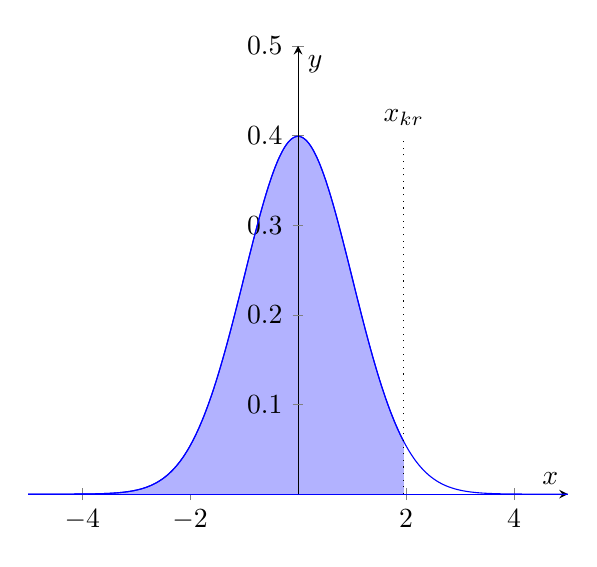
\begin{tikzpicture}
			\begin{axis}[
				xmin=-5, xmax=5, xlabel=$x$,
				ymin=0, ymax=.5, ylabel=$y$,
				samples=400,
				axis x line=middle,
				axis y line=middle,
				domain=-5:5,
				]
				\addplot[mark=none,smooth,blue] {1/sqrt(2*pi)*exp(-0.5*x^2)};
				\addplot[mark=none,smooth,blue] {0};
				
				\addplot[mark=none,smooth,blue,name path=A,domain=-5:1.96] {1/sqrt(2*pi)*exp(-0.5*x^2)};
				\addplot[mark=none,smooth,blue,name path=B,domain=-5:1.96] {0};
				
				\addplot[blue!30] fill between[of=A and B];
				
				\draw (axis cs: 0,0) -- (axis cs: 0,0.4);
				\draw[ultra thin,gray] (axis cs: -0.1,0.1) -- (axis cs: 0.1,0.1);
				\draw[ultra thin,gray] (axis cs: -0.1,0.2) -- (axis cs: 0.1,0.2);
				\draw[ultra thin,gray] (axis cs: -0.1,0.3) -- (axis cs: 0.1,0.3);
				
				\draw[dotted] (axis cs: 1.96,0) to (axis cs: 1.96,0.4) node[above] {$x_{kr}$};
				
			\end{axis}
		\end{tikzpicture}
	\end{center}
	Für den Taschenrechner ist das kein Problem, wir wählen das Untermenü \texttt{3:Inv. Normal-V.} aus, geben die Fläche und die Parameter der Normalverteilung ein und erhalten $\approx$ 1,96.
	
	\section*{Menü 9: Tabellen}
	\subsection*{In eine Formel viele Werte gleichzeitig einsetzen}
	
	Das Tabellenmenü gibt einem die Möglichkeit, für eine Formel (oder mehrere Formeln) Werte einzusetzen und direkt das Ergebnis anzuzeigen. Hier anhand der Weibull-Verteilung (\url{https://en.wikipedia.org/wiki/Weibull_distribution}),die aber in Statistik 2 nicht behandelt wird (die Verteilungen, die in Statistik 2 behandelt werden, können auch im Verteilungsmenü berechnet werden). Die Dichte der Weibull-Verteilung ist:
	\begin{align}
		f(x) = \begin{cases}
			\frac{k}{\lambda} \cdot\left(\frac{x}{\lambda}\right)^{k-1} \cdot \exp\left(-\left[\frac{x}{\lambda}\right]^k\right) & x\ge 0 \\
			0 & x < 0
		\end{cases} \notag
	\end{align}
	Sie hat zwei Parameter $k>0$ \textit{shape} und $\lambda > 0$ \textit{scale}. Wir wollen die Dichte der Weibull-Verteilung an mehreren Stellen für $k = 2$, $\lambda = 1$ berechnen. Im Menü 9 fragt der Taschenrechner gleich nach $f(x)$. Hier geben wir die Formel ein, für $x$ benutzen wir die \taste{$x$}-Taste oben rechts, also
	\begin{align}
		f(x) = 2\cdot x\cdot e^{-x^2} \notag
	\end{align}
	Nach dem Drücken auf \taste{=} werden wir nach $g(x)$ gefragt. Hier könnte man eine weitere Funktion eingeben, aber das wollen wir nicht. Also drücken wir wieder \taste{=}. Dann werden wir nach den Werten für $x$ gefragt. Man kann den Startwert und Endwert für $x$ angeben, sowie die Schrittlänge. Wir setzen für den Startwert 0, den Endwert setzen wir auf 3 und die Schrittweite (\textit{Inkre} abgekürzt) setzen wir auf 0.5. Wir erhalten folgende Tabelle:
	\begin{center}
		\begin{tabular}{c|c}
			$x$ & $f(x)$ \\
			\hline
			0 & 0 \\
			0.5 & 0.7788 \\
			1 & 0.7357 \\
			1.5 & 0.3161 \\
			2 & 0.0732 \\
			2.5 & $9.6 \cdot 10^{-3}$ \\
			3 & $7.4 \cdot 10^{-4}$
		\end{tabular}
	\end{center}
	
\end{document}